%!TEX root = main.tex

\section{The Implemented Symbolic Matrix Factorization}

\begin{frame}{Symbolic Matrix Factorization}{\acf{LU}}
  The ``standard'' in numerical linear algebra \dots
  \begin{bbox}[Full-Pivoting \acs{LU} Factorization]
    Given a matrix $\m{A} \in \mathbb{R}^{m \times n}$, with $m \geq n$, the full-pivoting \ac{LU} decomposition is defined as the process of decomposing $\m{A}$ into the product of
    \begin{itemize}
      \item a $\m{L} \in \mathbb{R}^{m \times m}$ lower-triangular matrix with all diagonal entries equal to $1$;
      \item a $\m{U} \in \mathbb{R}^{m \times n}$ upper-triangular matrix;
      \item a $\m{P} \in \mathbb{R}^{m \times m}$ and a $\m{Q} \in \mathbb{R}^{n \times n}$ matrices for rows and columns permutation;
    \end{itemize}
    such that $\m{P}\m{A}\m{Q} = \m{L}\m{U}$.
  \end{bbox}
  \dots It carries the minimum number of operations!
\end{frame}

\begin{frame}{Symbolic Matrix Factorization}{\acf{FFLU}}
  Trying to guarantee exact divisions on factors \dots
  \begin{bbox}[Full-Pivoting \acs{FFLU} Factorization]
    Given a matrix $\m{A} \in \mathbb{R}^{m \times n}$, with $m \geq n$, the full-pivoting \ac{FFLU} decomposition is defined as the process of decomposing $\m{A}$ into the product of
    \begin{itemize}
      \item a lower-triangular matrix $\m{L} \in \mathbb{R}^{m \times m}$ with all diagonal entries equal to $1$;
      \item \textcolor{fg_sl_color}{a diagonal matrix $\m{D} \in \mathbb{R}^{m \times m}$;}
      \item an upper-triangular matrix $\m{U} \in \mathbb{R}^{m \times n}$;
      \item a $\m{P} \in \mathbb{R}^{m \times m}$ and a $\m{Q} \in \mathbb{R}^{n \times n}$ matrices for rows and columns permutation;
    \end{itemize}
    such that $\m{P}\textcolor{fg_sl_color}{\m{D}}\m{A}\m{Q} = \m{L}\m{U}$.
  \end{bbox}
  \dots same effectiveness of \ac{LU} decomposition, but with a slightly different implementation!
\end{frame}

\section{Symbolic Finite Element Method}

\begin{frame}{Symbolic computation (2/4): Finite element method problem}
  \begin{itemize}
    \item Symbolic computation can be applied to the \textbf{finite element (FE) method}. \\[0.5em]
    \item \textbf{Stiffness matrix}, \textbf{load vector}, and \textbf{boundary conditions} are defined symbolically. \\[0.5em]
    \begin{equation*}
      \left[\begin{array}{cc}
        \mathbf{K}_{ff} & \mathbf{K}_{fs} \\[0.5em]
        \mathbf{K}_{sf} & \mathbf{K}_{ss}
      \end{array}\right] \left[\begin{array}{c}
        \mathbf{d}_{f} \\[0.5em]
        \mathbf{d}_{s}
      \end{array}\right] = \left[\begin{array}{c}
        \mathbf{f}_{f} \\[0.5em]
        \mathbf{f}_{s}
      \end{array}\right]
      \quad \xrightarrow[\text{method}]{\text{direct stiffness}} \quad
      \begin{array}{c}
        \mathbf{d}_{f} = \mathbf{K}_{ff}^{-1}\,\left(\mathbf{f}_{f} - \mathbf{K}_{fs}\,\mathbf{d}_{s}\right) \\[0.5em]
        \mathbf{f}_{s} = \mathbf{K}_{sf}\,\mathbf{d}_{f} + \mathbf{K}_{ss}\,\mathbf{d}_{s}
      \end{array}
    \end{equation*} \\[0.5em]
    \begin{enumerate}
      \item Possibility to \textbf{evaluate} the system \textbf{without} the need to ``\textbf{reassemble}'' the system. \\[0.5em]
      \item Parametric formulation allows us to \textbf{explore} radical design changes through \textbf{optimization}. \\[0.4em]
      \item The system can also be solved \textbf{symbolically}~\dots~if you are lucky enough \raisebox{-3.5pt}{\huge\trollface{}}.
    \end{enumerate}
  \end{itemize}
  \begin{center}\begin{minipage}{10.75cm}\begin{block}{}
    \centering
    FE method $\quad \xrightarrow[\text{computation}]{\text{symbolic}} \quad$ Symbolic FE method + \textcolor{mycolor5}{\textbf{A lot of flexibility!}}
  \end{block}\end{minipage}\end{center}
  \begin{itemize}
    \item We combined all these features in the \Maple{} \TrussMe{} library (open-source).
  \end{itemize}
\end{frame}

\begin{frame}{Symbolic computation (3/4): Linear algebra}
  \begin{itemize}
    \item Symbolic matrix factorization is used for the computation of the linear system \textbf{solutions}.
    \begin{equation*}
      \mathbf{d}_{f} = \mathbf{K}_{ff}^{-1}\,\left(\mathbf{f}_{f} - \mathbf{K}_{fs}\,\mathbf{d}_{s}\right)
    \end{equation*}
    \item There are several matrix factorizations, the best are those that \dots
    \\[0.5em]
    \begin{enumerate}
      \item are capable of preserving \textbf{sparsity};
      \\[0.5em]
      \item limit the \textbf{expression swell} phenomenon;
      \\[0.5em]
      \item guarantee \textbf{numerical stability} of the solution.
      \\[1.0em]
    \end{enumerate}
    \item \Maple{} matrix factorizations have \textbf{limited capabilities}. \\[1.0em]
    \item We developed the \ac{LAST} symbolic matrix factorization toolbox capable of \dots  \\[0.5em]
    \begin{enumerate}
      \item dealing with these \Maple{} issues; \\[0.5em]
      \item introducing \textbf{veiling variables} not to increase the expressions size (through \ac{LEM} toolbox); \\[0.5em]
      \item performing LU, Fraction-Free LU, QR, and Gauss-Jordan factorizations. \\[1.5em]
    \end{enumerate}
  \end{itemize}
\end{frame}

\begin{frame}{Symbolic computation (4/4): Mixed symbolic/numerical solution}
  \begin{itemize}
    \item Sometimes it is not possible to obtain a \textbf{symbolic} solution to problems because of \dots \\[0.5em]
    \begin{enumerate}
      \item capability of the symbolic kernel to handle \textbf{complicated} expressions; \\[0.5em]
      \item \textbf{non-linear} or mathematically \textbf{unsolvable} problems. \\[1.0em]
    \end{enumerate}
    \item Symbolic computation should be exploited as much as possible! \\[0.5em]
  \end{itemize}
  \begin{center}\begin{minipage}{13.1cm}\begin{block}{}
    \centering
    FE model $\quad \xrightarrow[\text{computation}]{\text{symbolic}} \quad$ \hspace*{1.05cm}\textcolor{mycolor2}{\textbf{Stop}}\hspace*{1.05cm} $\quad \xrightarrow[\text{generation}]{\text{code}} \quad$ \begin{minipage}[c]{0.27\linewidth}\begin{center}{\textbf{Efficient} numeric \\ FE model solution}\end{center}\end{minipage}
  \end{block}\end{minipage}\end{center}
  \begin{center}\begin{minipage}{13.1cm}\begin{block}{}
    \centering
    FE model $\quad \xrightarrow[\text{computation}]{\text{symbolic}} \quad$ \textcolor{mycolor5}{\textbf{Symbolic solution}} $\quad \xrightarrow[\text{generation}] {\text{code}} \quad$ \begin{minipage}[c]{0.27\linewidth}\begin{center}{\textbf{Greased-lightning-fast} \\ numeric evaluation!}\end{center}\end{minipage}
  \end{block}\end{minipage}\end{center}
  \begin{itemize}
    \item K\&C of suspensions are computed through a \textbf{mixed} symbolic/numerical approach.
  \end{itemize}
\end{frame}

% - - - - - - - - - - - - - - - - - - - - - - - - - - - - - - - - - - - - - - -

\begin{frame}{Suspensions symbolic modeling (1/3): Case study}
  The modeled suspension is a \textbf{double wishbone} suspension system of the \textbf{Formula SAE} vehicle of \emph{E-Agle Trento Racing Team} (University of Trento). \\[1.0em]
  \begin{center}
    \begin{minipage}[c]{0.65\textwidth}
      \centering
      %\includegraphics[width=1.0\textwidth]{./figures/render_all.pdf}
    \end{minipage}
    \hspace*{1em}
    \begin{minipage}[c]{0.25\textwidth}
      \centering
      %\includegraphics[width=1.0\textwidth]{./figures/fsae.jpeg}
    \end{minipage}
  \end{center}
\end{frame}

\begin{frame}{Suspensions symbolic modeling (2/3): Rigid multibody \& FE models}
  \begin{minipage}[c]{0.55\linewidth}
    \begin{itemize}
      \item The main idea is \dots \\[0.5em]
      \begin{enumerate}
        \item to \textbf{decouple} the rigid multibody and FE models of the suspension. \\[0.5em]
        \item that compliance contribution are \textbf{small}. \\[1.0em]
      \end{enumerate}
    \end{itemize}
    \begin{center}\begin{minipage}{7.0cm}\begin{block}{}
      \centering
      \textcolor{mycolor1}{\textbf{Decoupling the two models take advantage of the best of both worlds!}}
    \end{block}\end{minipage}\vspace{1.0em}\end{center}
    \begin{itemize}
      \item The computation sequence is \dots \\[0.5em]
      \begin{enumerate}
        \item integration step of the \textbf{rigid multibody}; \\[0.5em]
        \item resolution of the \textbf{symbolic FE} model; \\[0.5em]
        \item sum the two contributions to obtain the \textbf{total displacement}. \\[1.0em]
      \end{enumerate}
    \end{itemize}
  \end{minipage}
  \begin{minipage}[c]{0.40\linewidth}
    %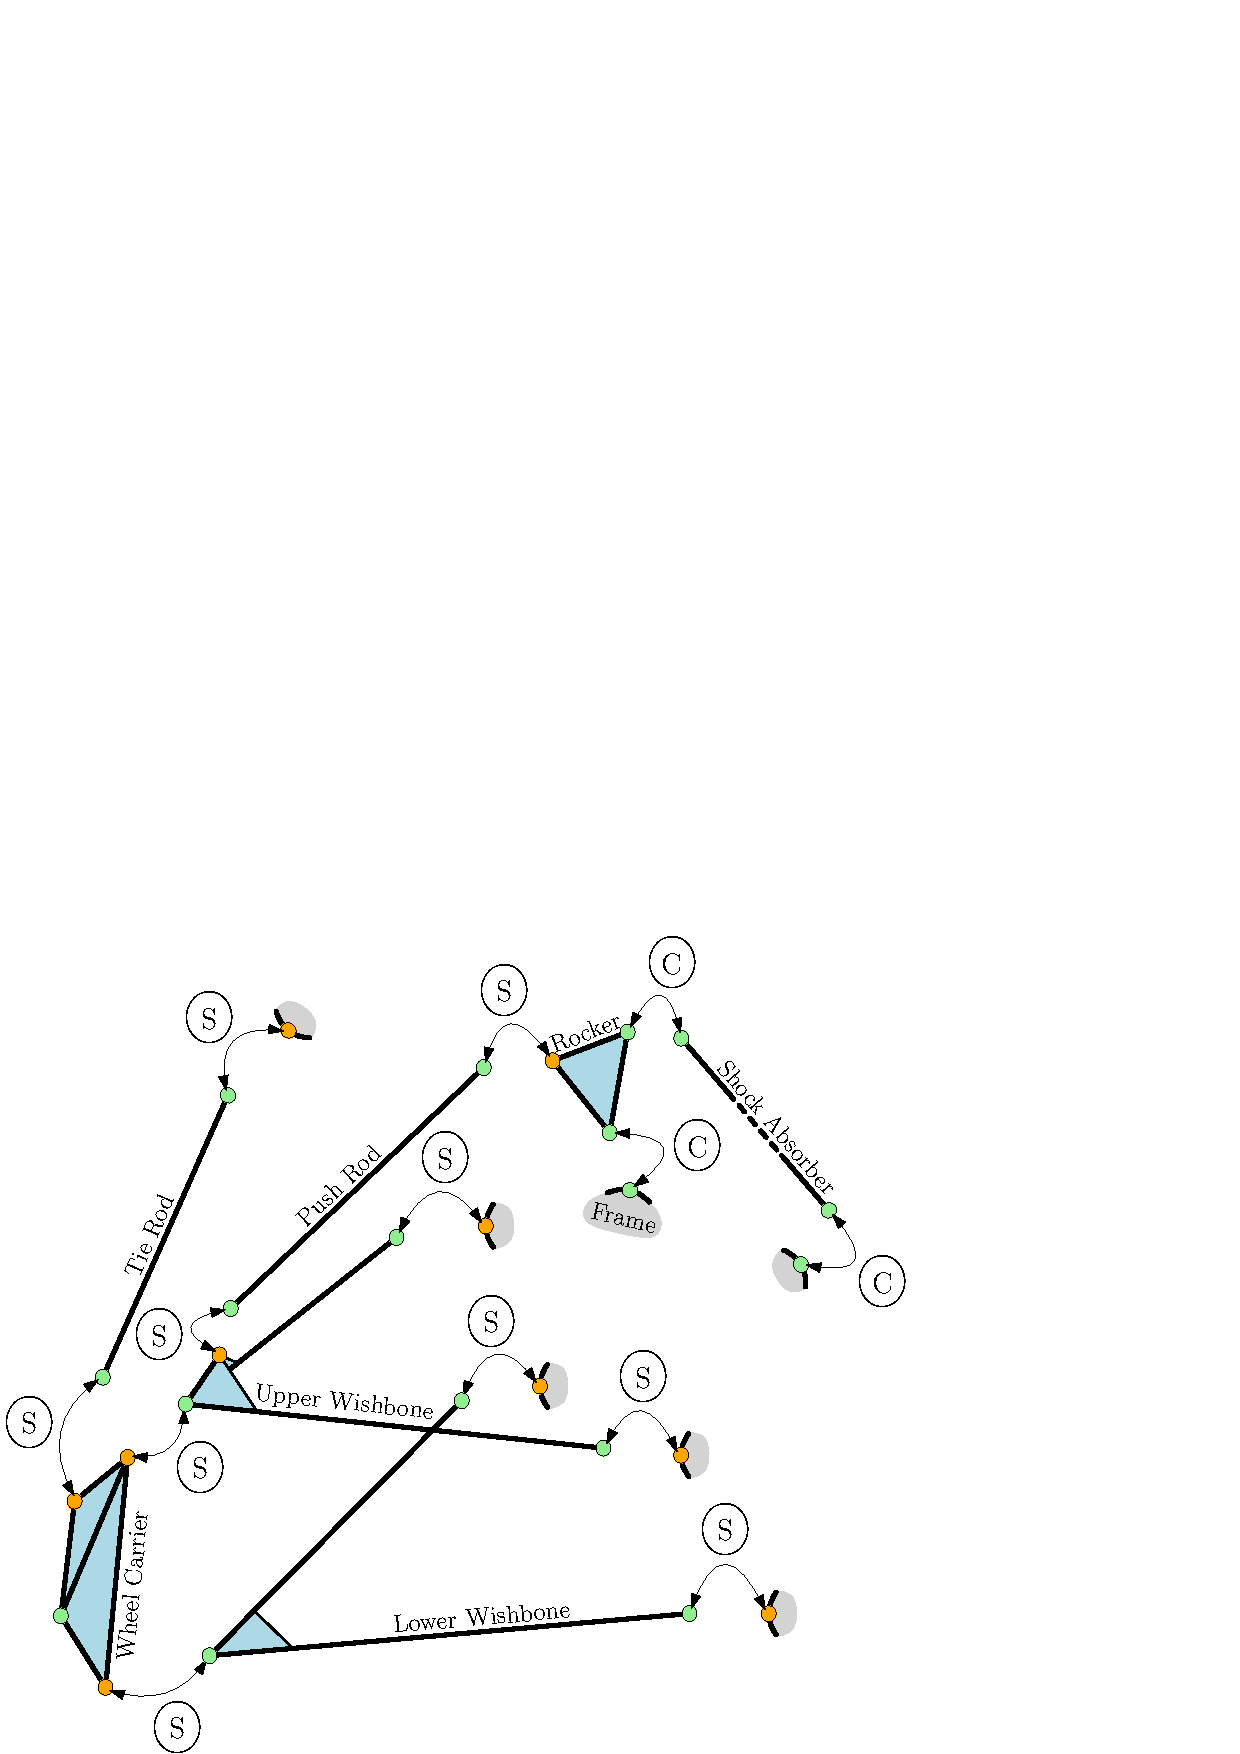
\includegraphics[width=1.0\textwidth]{./figures/constraints.pdf}
  \end{minipage}
\end{frame}

\begin{frame}{Suspensions symbolic modeling (3/3): \textcolor{mycolor2}{\textbf{Atenção! Perigo!}}}
  \centering{The \textbf{analytic frequency response} of the system is influenced by the \textbf{decoupling} strategy.} \\[0.5em]
  %\includegraphics[width=0.9\linewidth]{./figures/frequency_response.pdf}
  \begin{center}
    \emph{Legend:}
    {\color{mycolor1}$\blacksquare$} 1 DOF model, {\color{mycolor2}$\blacksquare$} 1 DOF + compliance contribution. \\[0.5em]
    \textcolor{mycolor5}{\textbf{Just be careful to the relation \fbox{$k_c \gg k$} and everything will be fine!}}
  \end{center}
\end{frame}

% - - - - - - - - - - - - - - - - - - - - - - - - - - - - - - - - - - - - - - -

\begin{frame}{Simulation results (1/4): Static analysis}
  %\centering{The \textbf{symbolic} solution with the \textbf{numerical} is compared with the one obtained with \Ansys{}.} \\[0.5em]
  \begin{center}
    \begin{minipage}[c]{0.485\linewidth}
      \centering{\textbf{Static translations}} \\[0.5em]
      %\includegraphics[width=1.0\textwidth]{./figures/static_translations.pdf}
    \end{minipage}
    \begin{minipage}[c]{0.485\linewidth}
      \centering{\textbf{Static rotations}} \\[0.5em]
      %\includegraphics[width=1.0\textwidth]{./figures/static_rotations.pdf}
    \end{minipage}
    \raggedright{\small{\emph{Legend:} \TrussMe{} solution (\emph{solid lines}), \Ansys{} data (\emph{bullets}). \\ {\color{mycolor1}$\blacksquare$} $F_x =$ \SI{4000}{\newton}, {\color{mycolor2}$\blacksquare$} $F_y =$ \SI{4000}{\newton}, {\color{mycolor3}$\blacksquare$} $F_z =$ \SI{4000}{\newton}, with $M_x = M_y = M_z =$ \SI{0}{\newton\meter}. \\ {\color{mycolor4}$\blacksquare$} $M_x =$ \SI{400}{\newton\meter}, {\color{mycolor5}$\blacksquare$} $M_y =$ \SI{400}{\newton\meter}, {\color{mycolor6}$\blacksquare$} $M_z =$ \SI{400}{\newton\meter}, with $F_x = F_y = F_z =$ \SI{0}{\newton}.}}
  \end{center}
\end{frame}

\begin{frame}{Simulation results (2/4): Design analysis examples}
  \centering{Usage examples of \textbf{design optimization} through the mixed numeric/symbolic solution.} \\[1.5em]
  \begin{center}
    \begin{minipage}[c]{0.475\linewidth}
      \centering{\textbf{Compliance optimization}} \\
      $\theta_z$ steer rotation of the carrier
      \\[0.5em]
      %\includegraphics[width=1.0\linewidth]{./figures/variation_compliance.pdf}
    \end{minipage}
    \begin{minipage}[c]{0.475\linewidth}
      \centering{\textbf{Loads optimization}} \\
      Axial force of the tie rod \\[0.5em]
      %\includegraphics[width=1.0\textwidth]{./figures/variation_force.pdf}
    \end{minipage}
  \end{center}
\end{frame}

\begin{frame}{Simulation results (3/4): Frequency response}
  The \textbf{frequency response} of the system is validated with the \Ansys{} \textbf{modal analysis} data. \\[1.0em]
  \begin{minipage}[c]{0.69\linewidth}
    \centering{\textbf{Acceleration/force frequency response}} \\[0.25em]
    %\includegraphics[width=1.0\linewidth]{./figures/frequency_response_simulations.pdf}
  \end{minipage}
  \hfill
  \begin{minipage}[c]{0.3\linewidth}
    %\includegraphics[width=0.5\linewidth]{./figures/mode1.png} \raisebox{2.0em}{$f = 7.6$ Hz} \\
    %\includegraphics[width=0.5\linewidth]{./figures/mode2.png} \raisebox{2.0em}{$f = 88.5$ Hz} \\
    %\includegraphics[width=0.5\linewidth]{./figures/mode3.png} \raisebox{2.0em}{$f = 159.7$ Hz} \\
  \end{minipage}
  \begin{center}
    \emph{Legend:}
    {\color{mycolor1}$\blacksquare$} \Ansys{}, {\color{mycolor2}$\blacksquare$} kinematic + compliance, {\color{mycolor3}$\blacksquare$} pure kinematic.
  \end{center}
\end{frame}

\begin{frame}{Simulation results (4/4): Timing}
  \begin{center}
    Real-time $=$ computation time $<$ $1$ ms step time \\[1.0em]
    %\includegraphics[width=0.8\textwidth]{./figures/timing.pdf} \\[2.0em]
    \textcolor{mycolor1}{\textbf{The mixed symbolic/numeric solution is capable of running under hard real-time!}} \\[2.0em]
  \end{center}
\end{frame}


% That's all Folks!